\whiteBGstarBegin
\setcounter{section}{0}

\begin{enumerate}[label=\bfseries Câu \arabic*:]
	\item \mkstar{1} [21]
	
	\cauhoi{
	Có một mặt phẳng diện tích $S$ được đặt trong từ trường đều $\vec B$. Khi các đường sức từ song song với mặt $S$ thì từ thông qua $S$ là
		\begin{mcq}(2)
			\item $\Phi = 0$. 
			\item $\Phi =-BS$.
			\item $\Phi = BS \cos \alpha$.
			\item $\Phi = BS$.
		\end{mcq}
	}
	\loigiai{
		
		\textbf{Đáp án: A.}	
		
	Khi các đường sức từ song song với mặt $S$ thì góc hợp bởi $\vec B$ và pháp tuyến $n$ là $90^\circ$ nên từ thông qua $S$ bằng 0.
		
	}
		\item \mkstar{2} [21]
		\cauhoi{
			
		Một khung dây dẫn hình chữ nhật có kích thước $3\ \text{(cm)}$ x $4\ \text{(cm)}$ được đặt trong từ trường đều cảm ứng từ $B = 5\cdot 10^{-4}\ \text T$. Vectơ cảm ứng từ hợp với mặt phẳng khung một góc $30^\circ$. Từ thông qua khung dây dẫn đó là
		
		\begin{mcq}(2)
			\item $3 \cdot 10^{-3}\ \text{Wb}$. 
			\item $3 \cdot 10^{-5}\ \text{Wb}$. 
			\item $3 \cdot 10^{-7}\ \text{Wb}$. 
			\item $6 \cdot 10^{-3}\ \text{Wb}$. 
		\end{mcq}
	}
	\loigiai{		
		
		\textbf{Đáp án: C.}	
		
		Góc hợp bởi $\vec B$ và $n$ là $60^\circ$.
	
		Từ thông qua khung dây dẫn đó là
		
		$$\Phi = NBS \cos \alpha = 3 \cdot 10^{-7}\ \text{Wb}.$$
	}
	\item \mkstar{1} [17]
	
	\cauhoi{
		Phát biểu định luật Faraday về suất điện động cảm ứng. Viết biểu thức, có chú thích và đơn vị.
		
	}
	
	\loigiai{		
		
		Định luật Faraday: Độ lớn suất điện động cảm ứng xuất hiện trong mạch kín tỉ lệ với tốc độ biến thiên từ thông qua mạch kín đó.
		
		$$|e_\text c| = \left|\dfrac{\Delta \phi}{\Delta t}\right|$$
		
		Với:
		
		+ $e_\text c$: Suất điện động cảm ứng (V),
		
		+ $\Delta \phi$: độ biến thiên từ thông (Wb),
		
		+ $\Delta t$: thời gian từ thông biến thiên qua mạch kín (s)
		
	}
	\item \mkstar{1} [37]
	
	\cauhoi{
		Viết công thức, nêu tên, đơn vị tính từ thông. Em hãy nêu ba cách làm biến đổi từ thông.
	}
	
	\loigiai{		
		
		$\Phi = NBS \cos \alpha$ 
		
		Với 
		+ $\alpha$ là góc giữa pháp tuyến $\vec n$ và $\vec B$, 
		
		+ $\Phi$: từ thông (Wb); 
		
		+ $N$: số vòng dây (vòng);
		
		+ $B$: cảm ứng từ (T); 
		
		+ $S$: diện tích vòng dây ($\text m^2$)
		
		- Thay đổi độ lớn $B$ của cảm ứng từ.
		 
		- Thay đổi độ lớn của diện tích $S$.
		
		- Thay đổi giá trị của góc $\alpha$.
		
		
	}
	\item \mkstar{2} [7]
	
	\cauhoi{
		Bếp từ hiện nay được sử dụng rộng rãi trong các hộ gia đình do có thể đun nấu nhanh, an toàn và tiết kiệm điện hơn những dòng bếp khác.
		\begin{enumerate}[label=\alph*)]
			\item Em hãy cho biết bếp từ hoạt động dựa trên hiện tượng Vật lý nào đã được học?
			\item Hãy định nghĩa hiện tượng Vật lý đó.
		\end{enumerate}	
		
	}
	
	\loigiai{
		
		\begin{enumerate}[label=\alph*)]
			\item Hiện tượng cảm ứng điện từ.
			\item Mỗi khi từ thông qua mạch kín biến thiên thì trong mạch kín xuất hiện một dòng điện gọi là dòng điện cảm ứng. Hiện tượng xuất hiện dòng điện cảm ứng trong mạch kín gọi là hiện tượng cảm ứng điện từ.
			
			Hiện tượng cảm ứng điện từ chỉ tồn tại trong khoảng thời gian mà từ thông qua mạch kín biến thiên.
		\end{enumerate}
		
	}

	\item \mkstar{2} [14]
	
	\cauhoi{
		Nhận tháng lương làm thêm đầu tiên, Khang đi siêu thị mua bộ nồi thủy tinh rất đẹp về tặng mẹ. Khi nấu ăn, mẹ Khang đặt nồi lên bếp từ nhưng mãi không đun nóng được, nhưng khi thay bằng nồi gang gia đình sử dụng trước đó thì lại đun được. Khang băn khoăn không hiểu tại sao. Bằng kiến thức Vật lí đã học, em hãy giải thích giúp Khang.
		
	}
	
	\loigiai{
		
		Các bếp từ chỉ sử dụng được với các loại xoong nồi, chảo có đáy bằng các kim loại có khả năng nhiễm từ hoặc vật liệu nhiễm từ (thép, gang, men sắt, thép không gỉ hoặc inox…), dòng điện Fu- cô sẽ làm cho đáy nồi sinh ra nhiệt rất lớn giúp nấu chín đồ ăn. Nồi thủy tinh không là vật liệu có khả năng nhiễm từ nên không sử dụng được với bếp từ. Do đó không đun nóng và làm chín đồ ăn được.
		
		
	}
	\item \mkstar{2} [7]
	
	\cauhoi{Một vòng dây giới hạn bởi diện tích $S = \SI{500}{cm}^2$ đặt trong từ trường đều có cảm ứng từ $B = \SI{0,1}{T}$. Biết vectơ $\vec B$ hợp với vectơ pháp tuyến của vòng dây một góc $60^\circ$.
		\begin{enumerate}[label=\alph*)]
			\item Tính từ thông qua diện tích $S$ của vòng dây.
			\item Nếu xoay cho vectơ $\vec B$ vuông góc với mặt phẳng vòng dây thì từ thông qua vòng dây lúc này có giá trị bao nhiêu?
		\end{enumerate}	
	}
	
	\loigiai{
		\begin{enumerate}[label=\alph*)]
			\item Từ thông qua diện tích $S$ của vòng dây
			
			$$\Phi = BS\cos \alpha = \text{2,5} \cdot 10^{-3}\ \text{Wb}.$$
			
			\item Nếu xoay cho vectơ $\vec B$ vuông góc với mặt phẳng vòng dây thì $\alpha = 0^\circ$.
			
			$$\Phi = BS\cos 0^\circ = \SI{0,005}{Wb}.$$
		\end{enumerate}	
	}
	
	\item \mkstar{2} [34]

	\cauhoi{
	Một khung dây hình chữ nhật có các cạnh $\SI{5}{cm}$ và $\SI{6}{cm}$ gồm 25 vòng đặt trong từ trường đều có cảm ứng từ $B = 4\cdot 10^{-2}\ \text T$. Pháp tuyến $\vec n$ của khung hợp với vectơ $\vec B$ góc $60^\circ$. Tính từ thông xuyên qua khung.
	}

	\loigiai{		
	
	Diện tích của khung dây
	
	$$S = ab = 30 \cdot 10^{-4}\ \text{m}^2.$$
	
	Từ thông xuyên qua khung
	
	$$\Phi =NBS \cos \alpha = \text{1,5} \cdot 10^{-3}\ \text{Wb}.$$
	}
	
	
	\item \mkstar{2} [12]
	
	\cauhoi{
		Hiện nay, bộ sạc không dây của nhiều dòng điện thoại Smartphone là ứng dụng hiện tượng dòng điện cảm ứng, phần đế sạc được cắm vào nguồn điện xoay chiều sẽ tạo ra một từ trường biến thiên $\vec B$, từ trường biến thiên này gởi qua cuộn dây được đặt sẵn trong chiếc điện thoại sẽ tạo ra từ thông biến thiên. Khi đó bên trong cuộn dây trong điện thoại sẽ xuất hiện từ trường cảm ứng $\vec B_\text c$ biến thiên, từ trường cảm ứng $\vec B_\text c$ biến thiên này sẽ tạo ra dòng điện cảm ứng $i_\text c$ trong cuộn dây, dòng điện này tất nhiên là sẽ được các mạch trong điện thoại điều chỉnh sao cho phù hợp với điện áp cho phép sạc của pin và chúng sẽ ngay lập tức sạc pin cho chiếc máy điện thoại .  
		Em hãy cho biết : 
		\begin{enumerate}[label=\alph*)]
			\item Nguyên tắc sạc không dây nói trên dựa vào hiện tượng Vật lí gì? 
			
			\item Theo em, nguyên nhân nào khiến cho công nghệ sạc không dây nói trên mất nhiều thời gian và hiệu năng thấp?
		\end{enumerate}	
	}
	
	\loigiai{
		
		\begin{enumerate}[label=\alph*)]
			\item Dựa vào hiện tượng cảm ứng điện từ.
			\item Vì khoảng một nửa từ trường gởi từ đế sạc sang điện thoại bị mất là nguyên nhân chính gây nên hiệu năng thấp và sạc pin lâu đầy. 
		\end{enumerate}	
	}
	
	\item \mkstar{2} [26]

		\cauhoi{
		Một khung dây hình vuông có cạnh $\SI{10}{cm}$ có điện trở $R = \SI{0,5}{\Omega}$, được đặt nghiêng góc $30^\circ$ so với của một từ trường đều với $B = \SI{0,02}{T}$.
		\begin{enumerate}[label=\alph*)]
			\item Tính từ thông gửi qua vòng dây đó.
			\item Từ trường tăng đều từ $B$ đến $2B$ trong khoảng thời gian $\SI{0,001}{s}$. Tính suất điện động cảm ứng xuất hiện trong vòng dây.
		\end{enumerate}	 
	
	
	}

	\loigiai{
	
	\begin{enumerate}[label=\alph*)]
		\item Góc hợp bởi $\vec B$ và $\vec n$ là $60^\circ$.
		
		Từ thông gửi qua vòng dây đó
		
		$$\Phi =NBS \cos \alpha  = 10^{-4}\ \text{Wb}.$$
		
		\item Suất điện động cảm ứng xuất hiện trong vòng dây
		
		$$ e_\text c = \dfrac{\Delta \Phi}{\Delta t} = \dfrac{N \Delta B S \cos \alpha }{\Delta t} =\SI{0,1}{V}.$$
	\end{enumerate}
	}
	
		\item \mkstar{2} [28]
	
	\cauhoi{
		Đặt một khung dây dẫn kín trong từ trường đều $\vec B$ như hình vẽ. Sự thay đổi độ lớn của từ trường đều B theo thời gian t được biểu diễn như đồ thị bên cạnh. Cho biết khoảng thời gian của các giai đoạn a, b, c, d, e là như nhau.
		\begin{center}
			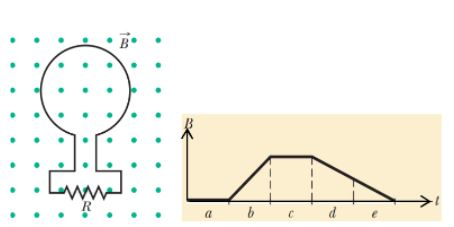
\includegraphics[scale=1]{../figs/VN11-2021-PH-TP024-01.JPG}
		\end{center}
		\begin{enumerate}[label=\alph*)]
		\item Hãy cho biết trong giai đoạn nào, suất điện động cảm ứng xuất hiện trong khung dây có độ lớn lớn nhất? Vì sao?
		
		\item Trong giai đoạn d, cho từ thông qua khung dây giảm đều từ $\SI{1,0}{Wb}$ xuống còn $\SI{0,5}{Wb}$ trong khoảng thời gian $\SI{0,1}{s}$. Tính độ lớn của suất điện động cảm ứng xuất hiện trong khung trong khoảng thời gian trên.
		\end{enumerate}
		
	}
	
	\loigiai{
		
		\begin{enumerate}[label=\alph*)]
		\item Suất điện động cảm ứng xuất hiện trong khung dây có độ lớn lớn nhất: giai đoạn b
		 
		\textbf{Giải thích}: Trong cùng một khoảng thời gian, giai đoạn b có độ biến thiên cảm ứng từ lớn nhất.
		
		\item Độ lớn của suất điện động cảm ứng xuất hiện trong khung
		
			$$|e_\text c| = \left|\dfrac{\Delta \phi}{\Delta t}\right| = \SI{5}{V}$$ 
		\end{enumerate}
	}
	
	
\end{enumerate}
\whiteBGstarEnd